\chapter{Nakamoto Consensus in Bitcoin}
\label{chpr:btc}
Bitcoin is a distributed, decentralized, peer-to-peer electronic payment system based on cryptographic proof instead of trust, allowing transactions between two counterparts without the need for a trusted third party. However, in late 2008, when the white paper was published by his author Satoshi Nakamoto\footnote{The name Satoshi Nakamoto is the pseudonym adopted by the creator of Bitcoin. While his identity remains a mystery, some information is known. He registered the domain bitcoin.org in August 2008 and in October 2008 he publicly released the famous white paper. In the Bitcoin's early days he participated extensively in forums and mailing lists maintaining the souce code. During the next two years other contributors slowly taken over the project maintenance and he stopped communicating, leaving a veil of mystery.}, it lacked a formalization of the protocol and of the guarantees it claimed to provide.

\bigskip
\noindent
This chapter delves into the core innovation behind Bitcoin, i.e. \textit{Nakamoto consensus}, term that is commonly used to refer to Bitcoin's novel consensus mechanism, which allows mutually distrusting pseudonymous identities to reach eventual agreement.

\bigskip
\section{Bitcoin \& Eventual Consistency}
By its very nature, the Bitcoin network is subject to a type of failure called \textit{network partition}, where a network splits into at least two parts that cannot communicate with each other, often due to software bugs, incompatible protocol versions, or simply network disconnections.
Thus, Bitcoin is inherently characterized by a trade-off between \textit{consistency}, \textit{availability} and \textit{partition tolerance}. Let us be more precise.
\begin{mydef} {\bf (consistency)}.
    All nodes in the system agree on the current state of the system.
\end{mydef}
\begin{mydef} {\bf (availability)}.
    The system is operational and instantly processing incoming requests.
\end{mydef}
\begin{mydef} {\bf (partition tolerance)}.
    Partition tolerance is the ability of a distributed system to continue operating correctly even in the presence of a network partition.
\end{mydef}

\bigskip
\noindent
In practice, only two of these properties can be reached simultaneously; a theorem by Brewer proves this result.
\begin{thm} {\bf (CAP theorem)}.
    It is impossible for a distributed system to simultaneously provide consistency, availability and partition tolerance. A distributed system can satisfy any two of these but not all three.
\end{thm}
\begin{proof}
    Let us assume two nodes that share some state. The nodes belongs to different partitions, so they cannot communicate each other. Assume a request wants to update the state and contacts one of the two nodes. The node may either: 1) update its local state, resulting in a situation of inconsistent states, or 2) not update, resulting in a system no longer available for updates.
\end{proof}

\bigskip
\noindent
Recalling the Definition \ref{def:consensus} of consensus and the properties it must satisfy, a clever intuition of Nakamoto is to weaken the agreement property to hold probabilistically and not deterministically, in order to deal with an asynchronous network. In particular the aforementioned trade-off is in advantage of partition tolerance rather than consistency. In fact, state changes of the underlying transaction ledger (i.e. the blockchain), are rendered probabilistic and the decision on a specific value of the state reaches $Pr(1)$ when $\lim_{r \to \infty}$, where $r$ is the number of rounds in the consensus protocol.

\bigskip
\noindent
Therefore, we can look at Bitcoin as an example of \textit{eventual consistency}.
\begin{mydef}{\bf (eventual consistency)}
    If no new updates to the shared state are issued, then eventually the system is in a quiescent state, i.e., no more messages need to be exchanged between nodes, and the shared state is consistent.
\end{mydef}

\bigskip
\noindent
Now that we have clear in mind the consensus problem from a computer science perspective, we must move forward and study how practically Nakamoto consensus works. Starting from a brief introduction of some basic Bitcoin mechanics we will dig into cryptography concepts and one another innovative idea: economic incentives in a consensus protocol.

\bigskip
\section{Bitcoin Design}
We already defined Bitcoin as a distributed, decentralized, peer-to-peer electronic payment system, but we lacked about defining the underlying digital asset, i.e. \textit{bitcoin}, and the challenges in building it, and also the fundamental bricks of the Bitcoin wall. Combining all these aspects is crucial to fully understand Nakamoto consensus.

\bigskip
\subsection{Constructing a Decentralized Digital Currency}
\textit{Ownership} is the first challenge of constructing a virtual currency. Imagine units of fiat currencies, their ownership depends on their form. If these units are in the form of paper notes or metal coins, ownership is simply determined by physical possession. Else, if these units are digitally stored in a bank account, ownership is determined by possession of the credentials to spend them. But what about ownership for a decentralized virtual currency? Who maintains the ledger of credentials? How can we guarantee the integrity of that ledger? In a network like Bitcoin nodes are free to leave at any time, thus a single source of trust (a node or a group of them) cannot be given this responsibility, even if one-way functions protects credentials. A solution could be that all nodes maintain a copy of that ledger, but what about validation? Can I feasible query all the nodes? Integrity is also crucial: usually digital signatures ensure it, but reminds the nodes could act maliciously and so, can I trust the signer?

\bigskip
\noindent
Another big challenge is the so called \textit{double spending} problem. This refers to the fact that the owner of some units of digital currency could spend them more than once. With fiat currencies, granted by a central authority, this problem cannot occur. In fact the bank database is the single source of truth with regard to the deposited amount of currency. Thus, spending with f.e. an online transfer, would immediately result in the rebalancing of that account to reflect the spend. However, in a peer-to-peer decentralized network some malicious agent could try to perform a double spend taking advantage of the delay in updating the shared ledger. An example will explain better.

\begin{figure}[!htbp]
    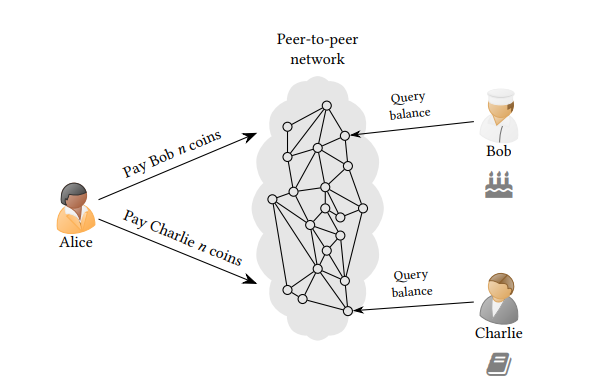
\includegraphics[width=1\linewidth]{Images/double-spending.png}
    \caption{Illustration of the double spending problem}
    \label{fig:double}
\end{figure}

\bigskip
\noindent
Consider the scenario described in Figure \ref{fig:double} where Alice tries to perform a double spend using some digital coins in her wallet. She would purchase a cake from Bob and a book from Charlie spending the same $n$ coins. For simplicity, let us assume that the two items cost the same, precisely $n$ units of currency. Thus, in order to finalize the purchase, both Bob and Charlie will provide Alice with their wallet addresses. Then Alice creates two different transactions, both spending the same $n$ coins, one paying Bob for the cake and the other paying Charlie for the book. The network will only accept one of them because the two transactions conflict. But there are several nodes in the network, some of which can be made to accept one of the transactions and the rest to accept the other. So Alice can transmit the transaction paying Bob to the portion of the network which Bob is connected to and the same argument holds for Charlie's transaction. Therefore, when Bob and Charlie query the balances in their private wallets they both will find a valid payment. If they provide Alice with their goods before being aware that the two transactions are conflicting, the result is that Alice has successfully performed a double spend.

\bigskip
\subsection{Bitcoin Mechanics}
Nakamoto solves brilliantly the aforementioned challenges in Bitcoin combining cryptography and social incentive engineering. But first we need a brief summary of the mechanics of the protocol.